% !TEX root = ../paper.tex

\section{UAV-TAlign-12K and Evaluation Protocol}

\subsection{Dataset Scope}

UAV-TAlign-12K is a benchmark for real captured UAV infrared-visible alignment. The collection
contains 6,039 synchronized RGB-infrared pairs, corresponding to 12,078 images across 15 scenes.
Its official evaluation split contains 6,037 integrity-checked pairs and 12,074 images. The
collection spans cross-FOV and cross-resolution sensing under day, night, and low-light capture,
grayscale and pseudocolor thermal rendering, and wide, zoom, and standard UAV views.

All journal-scale experiments use the same versioned manifest. UAV-TAlign-1K-Lite is retained as
a fixed development and ablation subset, while UAV-TAlign-12K defines the benchmark-scale
evaluation in this study. The official split comprises 7 day, 5 night, and 3 low-light scenes,
together with 8 grayscale-thermal and 7 pseudocolor-thermal scenes. Paired wide and zoom views
provide controlled cross-FOV comparisons within the substation scene family.

\begin{table}[t]
\caption{Positioning of UAV-TAlign-12K relative to representative infrared-visible and UAV
multimodal resources. UAVMatch denotes the synthetic transform-supervised UAV alignment
benchmark.}
\label{tab:dataset_positioning}
\centering
\resizebox{\textwidth}{!}{
\begin{tabular}{lllll}
\toprule
Resource & Data basis & Alignment signal & Scale & Primary evaluation focus \\
\midrule
KAIST / FLIR / LLVIP / M3FD & Ground or mixed RGB-infrared data & Paired or aligned imagery & Dataset-specific & Detection, fusion, low-light perception \\
DroneVehicle / VTUAV / LasHeR / Anti-UAV & UAV or tracking-centric RGB-infrared data & Task annotations & Dataset-specific & Detection or tracking under multimodal sensing \\
UAVMatch / TGRS~\cite{gao2025uavmatch} & Synthetic transforms from UAV multimodal data & Affine / homography supervision & 81K train / 15K test pairs & Supervised transform regression and geometric metrics \\
ATR-UMMIM~\cite{bin2025atrummim} & Real UAV visible / infrared / registered-visible triplets & Semi-automated pixel-level reference & 7,969 triplets & Pairwise registration accuracy and condition attributes \\
UAV-TIRVis~\cite{vasile2025uavtirvis} & Real UAV thermal-visible imagery & Manual pairwise registration & 80 pairs & Direct image-domain registration quality \\
UAV-TAlign-12K & Real captured cross-FOV UAV infrared-visible data & Multi-frame scene protocol & 6,039 candidate / 6,037 evaluated pairs & Pairwise evidence, scene consensus, and operating coverage \\
\bottomrule
\end{tabular}}
\end{table}

\begin{figure}[t]
\centering
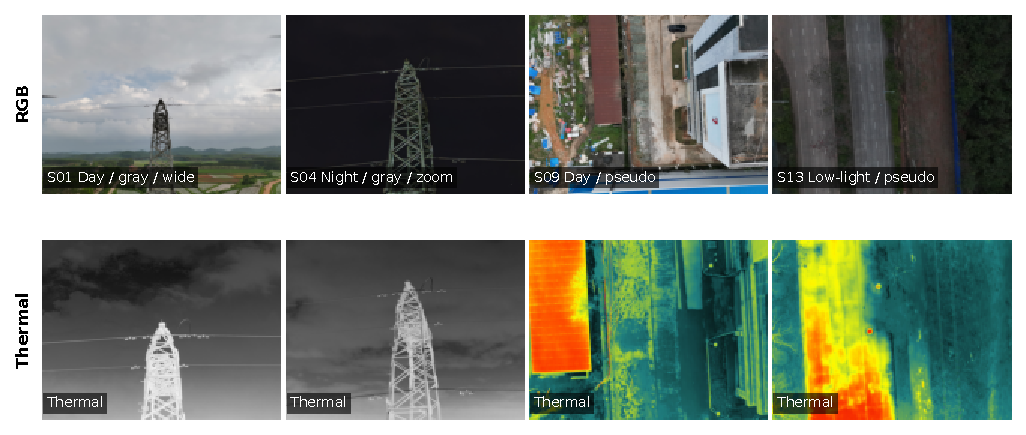
\includegraphics[width=\textwidth]{figures/fig_dataset_examples.pdf}
\caption{Representative UAV-TAlign-12K RGB-infrared pairs spanning illumination, thermal
rendering, and view conditions.}
\label{fig:dataset_examples}
\end{figure}

\subsection{Acquisition and Curation}

UAV-TAlign-12K was acquired between the second half of 2024 and the first half of 2026 across
industrial and natural scenes in southern China. All scenes were captured with the same DJI
Matrice 350 RTK platform and Zenmuse H30T multisensor payload. The integrated payload
automatically synchronized the visible and infrared products, preserving the native cross-sensor
geometry. The flights combined hovering and route-based capture using a registered aircraft, a
CAAC-qualified pilot, and permitted flight areas.

The released streams retain the native H30T acquisition modes. Wide-camera stills are
$4032\!\times\!3024$, zoom-camera stills are $3664\!\times\!2748$, and thermal images are
$1280\!\times\!1024$. In scenes 01 and 02, $3840\!\times\!2160$ still images were triggered while
H30T video recording was active. Scene 07 is a synchronized video-derived sequence sampled at
2 frames per second over one complete orbit around a transmission tower. Grayscale scenes use the
H30T \emph{White Hot} setting, and pseudocolor scenes use the on-device \emph{Hot Iron} palette.

Curation criteria were fixed before algorithm evaluation and covered scene relevance, exposure,
focus, and file integrity. The resulting candidate collection contains 6,039 synchronized pairs;
the integrity audit defines the 6,037-pair official evaluation split. Selection did not use matcher
outputs, alignment estimates, or quality scores.

Release preparation removes embedded metadata and normalizes filenames while preserving image
pixels. RGB and infrared files are linked through their shared H30T capture key, ordered by capture
time and sequence index, and assigned a common six-digit pair identifier. The release applies no
resizing, cropping, rotation, recompression, or image enhancement. Guangxi University owns the
collection, which is prepared for release under the Creative Commons Attribution 4.0 International
license.

\subsection{Dataset Organization}

Each scene has dedicated \texttt{rgb/} and \texttt{thermal/} directories, and paired samples share
the same filename stem. The official manifest records scene identity, pair identity, illumination,
thermal rendering, view type, and scene label. A scene groups frames sharing a site or target
context and acquisition condition. It may represent a continuous sequence or multiple sorties
under the same scene definition. Scene 07 is the documented single-orbit video sequence.

One manifest supports all pairwise, scene, and condition analyses. It also maps every reported
result to its source scene and pair identifier.

\subsection{Multi-Level Evaluation Protocol}

The benchmark defines three complementary tracks. Track A evaluates each of the 6,037 pairs
independently and measures the availability and support of pairwise homography evidence. Track B
aggregates frame estimates into a scene transform and reports the canonical set of high-confidence
scene products. Track C orders scenes with a fixed, interpretable reliability score to construct
coverage-aware operating profiles.

Together, the tracks connect matcher output to deployable scene geometry. Pairwise measurements
characterize evidence generation, scene-level measurements characterize multi-frame consensus,
and the operating profile exposes how product coverage changes with scene quality.

\subsection{Label-Free Scene-Consistency Diagnostics}

The protocol uses label-free relative signals for scalable scene-consistency analysis. The stored
diagnostics compare the optimized transform with its baseline initialization and quantify changes
in cross-modal agreement. They include edge-overlap improvement, gradient-NCC improvement, the
fraction of frames with improved gradient agreement, severe baseline-relative outlier count and
ratio, accepted-frame support, homography dispersion, and robust-rejection ratio.

These signals jointly characterize cross-modal improvement, geometric support, and consensus
stability. The resulting diagnostics support canonical product selection, condition-aware analysis,
and reliability--coverage visualization under a common evaluation interface
\cite{ma2021survey,liao2024survey}.
